\markboth{}{}
% Plus petite marge du bas pour la quatrième de couverture
% Shorter bottom margin for the back cover
\newgeometry{inner=20mm,outer=20mm,top=40mm,bottom=20mm}

%insertion de l'image de fond du dos (resume)
%background image for resume (back)
\backcoverheader

% Switch font style to back cover style
\selectfontbackcover{ % Font style change is limited to this page using braces, just in case


\noindent \textbf{Assistant engineering internship}\\
\begin{multicols}{2}[\columnsep2em] 
    \smallTwelve{
    \noindent \textbf{Intern}: Paul WALCZAK\\
    \noindent \textbf{Semester}: Semestre 8\\
    \noindent \textbf{Company}: Upteko ApS\\
    \noindent \textbf{Company tutor}:Vincent KLYVERTS TOFTERUP\\
    \noindent \textbf{ENIB tutor}: Alexis MICHEL\\
    }
    \columnbreak
    \hfill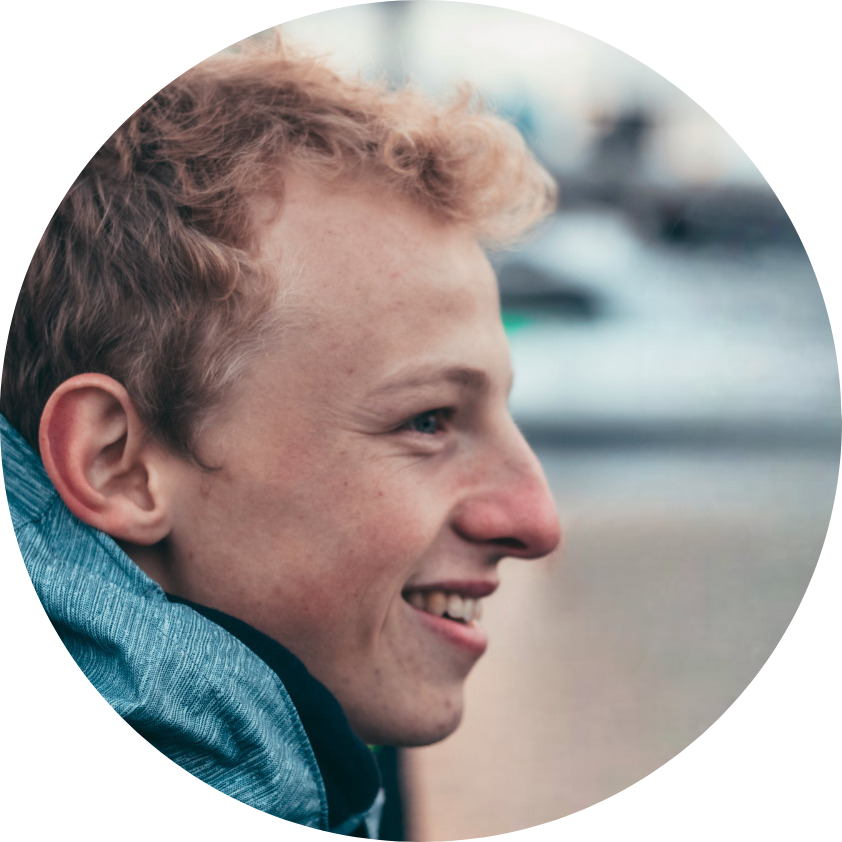
\includegraphics[keepaspectratio,height=3cm]{./cover/profile.png}
\end{multicols}


\subject{Mechatronics, robotics, embedded electronics, and software development} 

\keywords{STM32, drone, RTOS, embedded system, AHRS, telemetry} 

\compagny{Upteko is a rapidly growing company, founded in 2018 by Mads Joergensen, Benjamin Mejnertz, and Sebastian Duus, with a mission to develop drone applications for the maritime sector. The company's work environment is diverse and dynamic, encompassing various fields such as hardware, software, simulation, fundraising, and professional events. Upteko's primary innovation is a multipurpose drone system designed for maritime use, capable of performing a wide range of tasks autonomously. This system includes a drone and a charging station, allowing for 100$\%$ automatic ship inspections in less than two hours, among other functionalities. The company's flexible work culture, which includes the possibility of remote work, contributes to a positive and productive work environment. Despite its rapid growth, Upteko maintains a close-knit team of experienced drone pilots, software and hardware engineers, and business developers across its offices in Copenhagen, Odense, and Skanderborg.}

\resume{During my internship at Upteko, I had the opportunity to immerse myself in the world of drone technology through various projects. One of the main projects I worked on was the STM32 IMU project. The goal was to extract roll, pitch, and yaw data from the PModNav to create a 3D visualization of the IMU, which was crucial for tasks such as safety deployment and drone tracking. I managed to set up the STM32-L4796ZG to recover the sensor values from the PModNav and transmit them to the HMI. I also spent a significant amount of time migrating files in ROS2. Despite the complexity of the environment and the evolution of programming languages, I successfully migrated all the files. This task allowed me to learn valuable principles such as Quality Of Services and Micro Air Vehicle Link message communication. Additionally, I worked on a Software-In-The-Loop (SITL) project. This involved integrating TeraTowerEvo distance sensors into a simulation vehicle and parameterizing them for realistic operation. These projects not only deepened my understanding of drone technology but also allowed me to apply my academic knowledge to real-world problems. The experience was challenging but incredibly rewarding, and I am grateful for the opportunity.} 

\conclusion{My abroad internship provided me with a unique opportunity to apply my academic knowledge to real-world problems, particularly in the field of drone technology. Despite the occasional hurdles, the experience was invaluable, offering me a deeper understanding of the workings of a rapidly growing company and the complexities of working in a multifaceted environment. I am grateful for the skills I have acquired and the insights I have gained, and I look forward to applying these in my future career.}

\restoregeometry
}
